\begin{frame}
    \titlepage
\end{frame}


\tikzset{
    stackBox/.style={very thick},
    onStack/.style={thick},
    frameOne/.style={fill=blue!15},
    frameTwo/.style={fill=red!15},
    markLine/.style={blue!50!black},
    markLineB/.style={red!90!black},
    hiLine/.style={red!90!black},
}

\begin{frame}{on the homework}
    \begin{itemize}
        \item due Friday + 1 week
        \item questions?
        \vspace{.5cm}
        \item big hint in assignment: {\tt gets} is what does buffer overflow
        \item reading the assembly should be fairly straightforward
            \begin{itemize}
            \item probably easiest strategy in this case
            \end{itemize}
        \item debugger can find stack addresses you need
    \end{itemize}
\end{frame}

\section{Continuing beyond stacking smashing}

\begin{frame}{}
    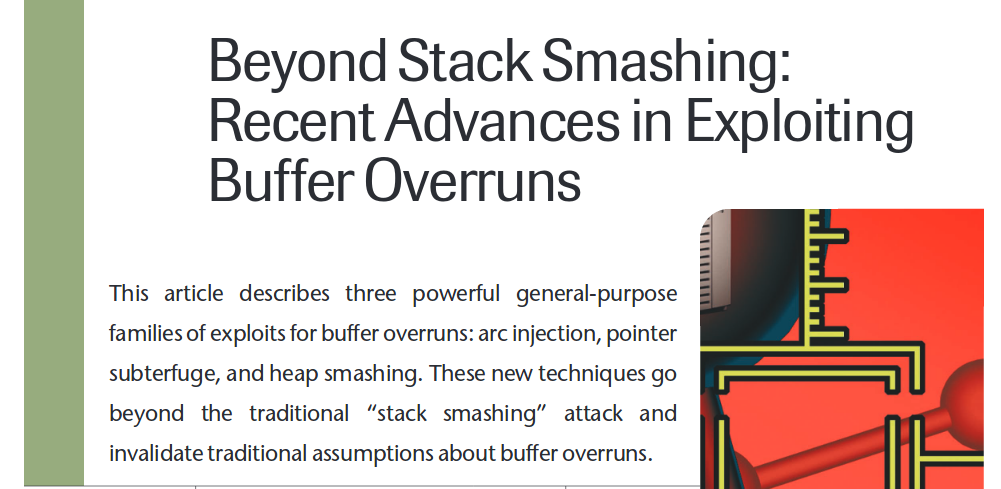
\includegraphics[width=\textwidth]{beyond-stack-smashing-title}
\end{frame}

\begin{frame}<1>[label=altExploits]{techniques from Pincus and Baker}
\begin{itemize}
\item \myemph<2>{arc injection} AKA return-oriented programming
    \begin{itemize}
    \item more detail (+ assignment) later in semester
    \end{itemize}
\item \myemph<3>{overwriting data pointers}
\item overwriting function pointers
\item overwriting pointers to function pointers
\item (on heap) overwriting {\tt malloc}'s data structures
\end{itemize}
\end{frame}

\begin{frame}{other buffer overflows?}
    \begin{itemize}
        \item examples last time:
        \vspace{.5cm}
        \item luck: ``\texttt{score}'' for quiz on stack next to answer
        \item ``arc injection'' --- return to existing code
        \item data pointer on stack
    \end{itemize}
\end{frame}

\againframe<2>{altExploits}

\subsection{arc injection}

\begin{frame}[fragile,label=returnToSomewhere]{return-to-somewhere}
\begin{tikzpicture}
% FIXME:
\tikzset{
    stackBox/.style={very thick},
    onStack/.style={thick},
}
\begin{scope}[xscale=0.75]
\draw[stackBox] (0, 0) rectangle (10, -6);
\draw[thick,-Latex] (10.25,-5) -- (10.25, -1) node [midway, below, sloped] {increasing addresses};
\node[at={(5, 0.1)},anchor=south] { highest address (stack started here)};
\node[at={(5, -6.1)},anchor=north] { lowest address (stack grows here)};

\draw[onStack] (0, -.25) rectangle (10, -1.25) node[midway,align=center,font=\small] (stackAddr)
     {return address for {\tt vulnerable}: \\ address of {\tt do\_useful\_stuff}};
\draw[onStack,fill=black!20] (0, -1.25) rectangle (10, -2.25) node[midway,align=center,font=\small] {unused space (20 bytes)};
\draw[onStack,fill=blue!20] (0, -2.25) rectangle (10, -5.25) node[midway,align=center,font=\small] {buffer (100 bytes)};

\draw[onStack] (0, -5.25) rectangle (10, -6) node[midway,align=center,font=\small] {return address for {\tt scanf}};

\draw[onStack,fill=red!20,opacity=0.9] (0, -5.25) rectangle (10, -1.25) node[midway,align=center,font=\small,text=red!50!black] {unused junk};

\draw[-Latex,red,ultra thick,dashed] ([yshift=2.5mm]stackAddr.south east) -- ++(.25cm,0cm) |-
    (11, -4.25) node[align=left,right,font=\small] { {\tt do\_useful\_stuff} \\ (already in program) };

\begin{visibleenv}<2>
\fill[white,opacity=0.5, overlay] (-1,-2) rectangle (18, -8);
\end{visibleenv}
\end{scope}
\end{tikzpicture}
\begin{tikzpicture}[overlay,remember picture]
\begin{visibleenv}<2>
\node[fill=white,draw,ultra thick,align=center,anchor=center] at (current page.center) {
    code is \myemph{already in program}??? \\
    how often does this happen??? \\
    \ldots turns out ``\myemph{usually}'' --- more later in semester
};
\end{visibleenv}
\end{tikzpicture}
\end{frame}

\subsection{pointer subterfuge}

\againframe<3>{altExploits}

\begin{frame}[fragile,label=pointerSub]{pointer subterfuge}
\lstset{
    language=C,
    style=small,
    moredelim={**[is][\btHL<2|handout:0>]{~2~}{~end~}},
    morekeywords={size_t},
}
\begin{lstlisting}
void f2b(void *arg, size_t len) {
    char buffer[100];
    long val = ...; /* assume on stack */
    long *ptr = ...; /* assume on stack */
    memcpy(buff, arg, len); /* overwrite ptr? */
    ~2~*ptr = val~end~; /* arbitrary memory write! */
}
\end{lstlisting}
\imagecredit{adapted from Pincus and Baker, Figure 2}
% FIXME: stack picture
\end{frame}

\begin{frame}<1-3>[label=arbWrite]{arbitrary memory write}
    \begin{itemize}
    \item bunch of scenarios that lead to \myemph{single arbitrary memory write}
    \item how can attacker exploit this?
    \vspace{.5cm}
    \item<2-> \myemph<3>{overwrite return address directly}
    \item<2-> \myemph<4>{overwrite other function/code address pointer?}
    \item<2-> overwrite existing machine code (insert jump?)
    \item<2-> overwrite another data pointer --- copy more?
    \end{itemize}
\end{frame}

\begin{frame}[fragile,label=skipCanary]{skipping the canary}
\begin{tikzpicture}
% FIXME:
\tikzset{
    stackBox/.style={very thick},
    onStack/.style={thick},
}
\begin{scope}[xscale=1.2]
\draw[stackBox] (0, 0) rectangle (10, -6);
\draw[thick,-Latex] (10.25,-5) -- (10.25, -1) node [midway, below, sloped] {increasing addresses};
\node[at={(5, 0.1)},anchor=south] { highest address (stack started here)};
\node[at={(5, -6.1)},anchor=north] { lowest address (stack grows here)};

\draw[onStack] (0, -.25) rectangle (10, -1.25) node[midway,align=center,font=\small] (stackAddr)
     {return address for {\tt f2b} };
\draw[onStack,fill=red!20] (0, -1.25) rectangle (10, -2.25) node[midway,align=center,font=\small] (canaryAddr)
     {stack canary};
\draw[onStack,fill=green!20] (0, -2.25) rectangle (10, -2.75) node[midway,align=center,font=\small] (ptr) {ptr (8 bytes)};
\draw[onStack,fill=green!20] (0, -2.75) rectangle (10, -3.25) node[midway,align=center,font=\small] (val) {val (8 bytes)};
\draw[onStack,fill=blue!20] (0, -3.25) rectangle (10, -5.25) node[midway,align=center,font=\small] {buffer (100 bytes)};

\draw[onStack] (0, -5.25) rectangle (10, -6) node[midway,align=center,font=\small] {return address for {\tt scanf}};

\begin{visibleenv}<2->
\draw[-Latex,orange,ultra thick] ([xshift=1cm]ptr.east) -- ++(2cm,0cm) |- (stackAddr.east);
\draw[-Latex,orange,ultra thick,dashed] ([xshift=1cm]val.east) -- ++(2cm,0cm) |- (0.25, -5);
\end{visibleenv}

\begin{visibleenv}<3>
\draw[-Latex,red,ultra thick] ([yshift=2.5mm]stackAddr.south east) -- ++(.25cm,0cm) |- (0.25, -5);
\node[anchor=south west,red] at (0.25, -4.75) {
    machine code for the attacker to run
};
\end{visibleenv}
\end{scope}

\end{tikzpicture}
\end{frame}

\begin{frame}{fragility}
\begin{itemize}
\item problem: need to know exact address of return address
\item discussed how stack location varies --- this is tricky/unreliable
\end{itemize}
\end{frame}

\againframe<4>{arbWrite}

\begin{frame}[fragile,label=funcPtrQ]{function pointers?}
\lstset{language=C,style=small}
\begin{lstlisting}
int (*compare)(char *, char *);

if (sortCaseSensitive) {
    compare = compareStringsExactly;
} else {
    compare = compareStringsInsensitive;
}
...
if ((*compare)(string1, string2) == CMP_LESS) {
    ...
}
\end{lstlisting}
\end{frame}

\begin{frame}<2>[label=funcPtrCommon]{function pointers are common?}
    \begin{itemize}
    \item \myemph<2>{used in dynamic linking (stubs!)}
    \item \myemph<3>{in large C projects}
    \item \myemph<4>{used to implement C++ virtual functions}
    \end{itemize}
\end{frame}

\begin{frame}[fragile,label=dynStub]{dynamic linking stubs}
\begin{Verbatim}[fontsize=\fontsize{9}{10}\selectfont]
00000000004004a0 <__printf_chk@plt>:
  4004a0:       ff 25 82 0b 20 00       jmpq   *0x200b82(%rip)      
                                             # 601028 <_GLOBAL_OFFSET_TABLE_+0x28>
  4004a6:       68 02 00 00 00          pushq  $0x2
  4004ab:       e9 c0 ff ff ff          jmpq   400470 <_init+0x28>
\end{Verbatim}
\begin{itemize}
\item jumps to \texttt{\_GLOBAL\_OFFSET\_TABLE[5]}
\item \texttt{\_GLOBAL\_OFFSET\_TABLE[5]} \myemph{always} at address \texttt{0x601028}
\item \texttt{\_GLOBAL\_OFFSET\_TABLE[5]} is probably writeable
    \begin{itemize}
    \item if lazy binding --- normally updated first time printf called
    \end{itemize}
\end{itemize}
\end{frame}

\begin{frame}[fragile,label=gotOverwrite]{attacking the GOT}
\begin{tikzpicture}
% FIXME:
\tikzset{
    stackBox/.style={very thick},
    onStack/.style={thick},
}
\draw[stackBox] (0, 0) rectangle (10, -6);
\draw[thick,-Latex] (10.25,-5) -- (10.25, -1) node [midway, below, sloped] {increasing addresses};
\node[at={(5, 0.1)},anchor=south] { highest address (stack started here)};
\node[at={(5, -6.1)},anchor=north] { lowest address (stack grows here)};

\draw[onStack] (0, -.25) rectangle (10, -1.25) node[midway,align=center,font=\small] (stackAddr)
     {return address for {\tt f2b} };
\draw[onStack,fill=red!20] (0, -1.25) rectangle (10, -2.25) node[midway,align=center,font=\small] (canaryAddr)
     {stack canary};
\draw[onStack,fill=green!20] (0, -2.25) rectangle (10, -2.75) node[midway,align=center,font=\small] (ptr) {ptr (8 bytes)};
\draw[onStack,fill=green!20] (0, -2.75) rectangle (10, -3.25) node[midway,align=center,font=\small] (val) {val (8 bytes)};
\draw[onStack,fill=blue!20] (0, -3.25) rectangle (10, -5.25) node[midway,align=center,font=\small] {buffer (100 bytes)};

\draw[onStack] (0, -5.25) rectangle (10, -6) node[midway,align=center,font=\small] {return address for {\tt scanf}};

\node[anchor=south] at (13.5, -1) { global offset table };
\draw[stackBox] (11.5, -1) rectangle (15.25, -1.5) node[midway,font=\small] (printfEntry) {GOT entry: printf };
\draw[stackBox] (11.5, -1.5) rectangle (15.25, -2) node[midway,font=\small] {GOT entry: fopen };
\draw[stackBox] (11.5, -2) rectangle (15.25, -2.5) node[midway,font=\small] {GOT entry: exit };

\begin{visibleenv}<2->
\draw[-Latex,orange,ultra thick] ([xshift=1cm]ptr.east) -- ++(2cm,0cm) |- (printfEntry.west);
\draw[-Latex,orange,ultra thick,dashed] ([xshift=1cm]val.east) -- ++(2cm,0cm) |- (0.25, -5);
\end{visibleenv}

\begin{visibleenv}<3>
\draw[-Latex,red,ultra thick] ([yshift=2.5mm]printfEntry.south east) -- ++(.25cm,0cm) |- (0.25, -5);
\node[anchor=south west,red] at (0.25, -4.75) {
    machine code for the attacker to run
};
\end{visibleenv}
\end{tikzpicture}
\end{frame}

\againframe<3>{funcPtrCommon}

\begin{frame}[fragile,label=kernelFTbl]{function pointer tables: Linux kernel (1)}
\lstset{
    language=C,style=small,
    moredelim={**[is][\btHL<1|handout:0>]{~1~}{~end~}},
}
\begin{lstlisting}
struct file {
    union {
        struct llist_node       fu_llist;
        struct rcu_head         fu_rcuhead;
    } f_u;
    struct path             f_path;
    struct inode            *f_inode;       /* cached value */
    ~1~const struct file_operations    *f_op;~end~

    /*
     * Protects f_ep_links, f_flags.
     * Must not be taken from IRQ context.
     */
    spinlock_t              f_lock;
    atomic_long_t           f_count;
    ...
};
\end{lstlisting}
\end{frame}

\begin{frame}[fragile,label=kernelFTbl2]{function pointer tables: Linux kernel (2)}
\lstset{
    language=C,style=small,
    moredelim={**[is][\btHL<1|handout:0>]{~1~}{~end~}},
}
\begin{lstlisting}
struct file_operations {
    struct module *owner;
    loff_t (*llseek) (struct file *, loff_t, int);
    ssize_t (*read) (struct file *, char __user *,
                     size_t, loff_t *);
    ssize_t (*write) (struct file *, const char __user *,
                      size_t, loff_t *);
    ssize_t (*read_iter) (struct kiocb *, struct iov_iter *);
    ssize_t (*write_iter) (struct kiocb *, struct iov_iter *);
    int (*iterate) (struct file *, struct dir_context *);
    ...
};
\end{lstlisting}
\end{frame}

\againframe<4>{funcPtrCommon}

% FIXME: C++ vtables

\begin{frame}[fragile,label=CPPVirt]{C++ inheritence}
\lstset{
    language=C++,style=smaller,
}
    \vspace{-.5cm}
\begin{lstlisting}
class InputStream {
public:
    virtual int get() = 0;
    // Java: abstract int get();
    ...
};
class SeekableInputStream : public InputStream {
public:
    virtual void seek(int offset) = 0;
    virtual int tell() = 0;
};
class FileInputStream : public InputStream {
public:
    int get();
    void seek(int offset);
    int tell();
    ...
};
\end{lstlisting}
\end{frame}

\begin{frame}<1>[label=inheritMemLay]{C++ inheritence: memory layout}
\begin{tikzpicture}
    \tikzset{
        vt/.style={fill=blue!30},
    }
    \matrix[tight matrix,nodes={text width=3.8cm,text depth=.1ex,font=\small\tt},
            label={north:InputStream},anchor=north west] (inputStream)  at (0, 0) {
        |[vt]| vtable pointer \\
    };
    \matrix[tight matrix,nodes={text width=3.8cm,text depth=.1ex,font=\small\tt},
            label={north:SeekableInputStream},anchor=north west] (seekableStream) at (4.5, 0) {
        |[vt]| vtable pointer \\
    };
    \matrix[tight matrix,nodes={text width=6cm,text depth=.1ex,font=\small\tt},
            label={north:FileInputStream},anchor=north west] (fileStream) at (9, 0) {
        |[vt]| vtable pointer \\
        file\_pointer \\
    };
    \matrix[tight matrix,nodes={text width=3.8cm,text depth=.1ex,font=\small\tt},anchor=north west] (isVT) at (0, -2) {
        \tt slot for get\\
    };
    \matrix[tight matrix,nodes={text width=3.8cm,text depth=.1ex,font=\small\tt},anchor=north west] (seekVT) at (4.5, -2){
        \tt slot for get \\
        \tt slot for seek \\
        \tt slot for tell \\
    };
    \matrix[tight matrix,nodes={text width=6cm,text depth=.1ex,font=\small\tt},anchor=north west] (fileVT) at (9, -2){
        FileInputStream::get \\
        FileinputStream::seek \\
        FileInputStream::tell \\
    };
    \draw[thick,-Latex] (inputStream-1-1.east) -- ++(.35cm,0cm) |- (isVT-1-1.east);
    \draw[thick,-Latex] (seekableStream-1-1.east) -- ++(.35cm,0cm) |- (seekVT-1-1.east);
    \draw[thick,-Latex] (fileStream-1-1.east) -- ++(.35cm,0cm) |- (fileVT-1-1.east);
\end{tikzpicture}
\end{frame}

\begin{frame}[fragile,label=CPPImpl]{C++ implementation (pseudo-code)}
\lstset{
    language=C,style=smaller,
}
\vspace{-.5cm}
\begin{lstlisting}
struct InputStream_vtable {
    int (*get)(InputStream* this);
};

struct InputStream {
    InputStream_vtable *vtable;
};

...

    InputStream *s = ...;
    int c = (s->vtable->get)(s);
\end{lstlisting}
\end{frame}

\begin{frame}[fragile,label=CPPImplB]{C++ implementation (pseudo-code)}
\lstset{
    language=C,style=smaller,
}
\vspace{-.5cm}
\begin{lstlisting}
struct SeekableInputStream_vtable {
    struct InputStream_vtable as_InputStream;
    void (*seek)(SeekableInputStream* this, int offset);
    int (*tell)(SeekableInputStream* this);
};

struct FileInputStream {
    SeekableInputStream_vtable *vtable;
    FILE *file_pointer;
};

...

    FileInputStream file_in = { the_FileInputStream_vtable,  ... };
    InputStream *s = (InputStream*) &file_in;
\end{lstlisting}
\end{frame}

\begin{frame}[fragile,label=CPPImplC]{C++ implementation (pseudo-code)}
\lstset{
    language=C,style=smaller,
}
\vspace{-.5cm}
\begin{lstlisting}
SeekableInputStream_vtable the_FileInputStream_vtable = {
    &FileInputStream_get,
    &FileInputStream_seek,
    &FileInputStream_tell,
};

...

    FileInputStream file_in = { the_FileInputStream_vtable,  ... };
    InputStream *s = (InputStream*) &file_in;
\end{lstlisting}
\end{frame}



\begin{frame}{attacking function pointer tables}
% FIXME: picture
\begin{itemize}
\item option 1: overwrite table entry directly  
    \begin{itemize}
    \item required/easy for Global Offset Table --- fixed location
    \item usually not possible for VTables --- read-only memory
    \end{itemize}
\item option 2: create table in buffer (big list of pointers to shellcode), point to buffer
    \begin{itemize}
    \item useful when table pointer next to buffer
    \item (e.g. C++ object on stack next to buffer)
    \end{itemize}
\end{itemize}
\end{frame}

\section{NTP Exploit Case Study}

\begin{frame}[fragile,label=ntpStudyIntro]{case study (simplified)}
    \begin{itemize}
    \item bug in NTPd (Network Time Protocol Daemon)
    \item via Stepher R\"ottger, ``Finding and exploiting ntpd vulnerabilities''
    \end{itemize}
\lstset{
    language=C,
    style=small,
    moredelim={**[is][\btHL<1|handout:0>]{~1~}{~end~}},
    moredelim={**[is][\btHL<2|handout:0>]{~2~}{~end~}},
}
\begin{lstlisting}
static void
ctl_putdata(
  const char *dp,
  unsigned int dlen,
  int bin   /* set to 1 when data is binary */
  ) {
    ...
    ~1~memmove((char *)datapt, dp, (unsigned)dlen);~end~
    datapt += dlen;
    datalinelen += dlen;
}
\end{lstlisting}
\end{frame}

\begin{frame}<1>[fragile,label=target]{the target}
\lstset{
    language=C,
    style=small,
    moredelim={**[is][\btHL<1|handout:0>]{~1~}{~end~}},
    moredelim={**[is][\btHL<2|handout:0>]{~2~}{~end~}},
}
\begin{lstlisting}
    memmove((char *)~1~datapt~end~, dp, (unsigned)dlen);
\end{lstlisting}
\begin{tikzpicture}
\tikzset{box/.style={thick}}
\draw[box,fill=blue!20] (0, 0) rectangle (10, -0.5) node[midway] (datapt) {datapt (global variable)};
\draw[box,fill=green!20] (0, -0.5) rectangle (10, -1.5) node[midway] {(other global variables)};
\draw[box,fill=red!20] (0, -1.5) rectangle (10, -2.5) node[midway] (buffer) {buffer (global array)};
\begin{visibleenv}<1-2>
    \draw[very thick,violet!70!black,-Latex] (datapt.west) -- ++(-.5cm,0cm) -| (0.5, -1.75);
\end{visibleenv}
\begin{visibleenv}<2->
    \draw[box,fill=orange!20] (11, -1) rectangle (15, -1.5) node[midway] (strlen) {strlen GOT entry};
\end{visibleenv}
\begin{visibleenv}<3->
    \fill[pattern=north west lines,pattern color=red,opacity=0.4] (0, -2.5) rectangle (10, 0);
    \draw[-Latex,very thick,dashed,red] (datapt) -| ([xshift=-0.5cm]strlen.west) -- (strlen.west);
\end{visibleenv}
\begin{visibleenv}<4->
    \draw[box,fill=violet!20] (11, -3) rectangle (15, -3.5) node[midway] (system) {{\tt system()} stub};
    \fill[pattern=north west lines,pattern color=red,opacity=0.4] (11, -1) rectangle (15, -1.5);
    \draw[-Latex,very thick,dashed,red] (strlen.south) -- (system.north);
\end{visibleenv}
\end{tikzpicture}
\end{frame}

\begin{frame}[fragile,label=moreContext]{more context}
\lstset{
    language=C,
    moredelim={**[is][\btHL<1|handout:0>]{~1~}{~end~}},
    moredelim={**[is][\btHL<2|handout:0>]{~2~}{~end~}},
}
\begin{lstlisting}
    memmove((char *)~1~datapt~end~, dp, (unsigned)dlen);
    ...
    ...
    strlen(some_user_supplied_string)
    /* calls strlen@plt
       looks up global offset table entry! */
\end{lstlisting}
\end{frame}

\againframe<2>{target}

\begin{frame}{overall exploit}
    \begin{itemize}
    \item overwrite {\tt datapt} to point to strlen GOT entry
    \item overwrite value of strlen GOT entry
    \item example target: {\tt system} function
            \begin{itemize}
                \item executes command-line command specified by argument
            \end{itemize}
    \item supply string to provide argument to ``{\tt strlen}''
    \end{itemize}
\end{frame}

\againframe<3->{target}

\begin{frame}{overall exploit: reality}
    \begin{itemize}
    \item real exploit was more complicated
    \item needed to defeat more mitigations
    \item needed to deal with not being able to write {\tt \textbackslash 0}
    \item actually tricky to send things that trigger buffer write
        \begin{itemize}
        \item (meant to be local-only)
        \end{itemize}
    \end{itemize}
\end{frame}

% FIXME: interger overflow

% FIXME: heap smashing

% FIXME: use-after-free



\begin{frame}<1>[label=errorTypes]{beyond normal buffer overflows}
    \begin{itemize}
    \item pretty much every memory error is a problem
    \item will look at exploiting:
    \item \myemph<2>{off-by-one buffer overflows (!)}
    \item \myemph<3>{heap buffer overflows}
    \item \myemph<5>{double-frees}
    \item \myemph<4>{use-after-free}
    \item \myemph<6>{integer overflows in size calculations}
    \end{itemize}
\end{frame}

\againframe<2>{errorTypes}

\begin{frame}[fragile,label=prelim]{preliminaries}
    \begin{itemize}
    \item \myemph{frame pointers} are commonly used in addition to stack pointers
    \item not something we've seen in x86-64 assembly
    \end{itemize}
\end{frame}

\begin{frame}{frame pointers}
\begin{tikzpicture}
\tikzset{
    stackBox/.style={very thick},
    onStack/.style={thick},
}
\draw[stackBox] (0, 0) rectangle (8, -6);
\draw[thick,-Latex] (-.25,-5) -- (-.25, -1) node [midway, above, sloped] {increasing addresses};
\draw[onStack] (0, -.25) rectangle (8, -1.25) node[midway,align=center,font=\small] (retFoo)
    { return address for {\tt foo} };
\draw[onStack,frameOne] (0, -1.25) rectangle (8, -2.25) node[midway,align=center,font=\small] (saveFoo)
    { saved {\tt \%rbp} };
\draw[onStack,frameOne] (0, -2.25) rectangle (8, -5.25) node[midway,align=center,font=\small] (localFoo)
    { local variables for {\tt foo} };
\draw[Latex-,very thick,markLine] (8, -1.25) -- ++(1.5cm,0cm) node[right] {{\tt \%rbp} within {\tt foo}};
\draw[Latex-,very thick,markLine] (8, -5.25) -- ++(1.5cm,0cm) node[right] {{\tt \%rsp} within {\tt foo}};
\end{tikzpicture}
\end{frame}


\begin{frame}[fragile,label=fpCode]{frame pointer code}
\lstset{
    language=myasm,
    style=small
}
\begin{tikzpicture}
\node[draw] (manualFP) {
\begin{lstlisting}
foo:
  // prologue
  pushq %rbp
  movq %rsp, %rbp
  subq $120, %rsp
  ...
  ...
  ...
  movq %rbp, %rsp
  popq %rbp
  ret
\end{lstlisting}
};
\node[draw, left=.5cm of manualFP] (autoFP) {
\begin{lstlisting}
foo:
  // prologue
  pushq %rbp
  enter $120, $1
  ...
  ...
  ...
  leave
  ret
\end{lstlisting}
};
\node[draw, right=.5cm of manualFP] (noFP) {
\begin{lstlisting}
foo:
  // prologue
  sub $120, %rsp
  ...
  ...
  ...
  add $120, %rsp
  ret
\end{lstlisting}
};
\end{tikzpicture}
\end{frame}

\begin{frame}{stack layout: two functions}
\begin{tikzpicture}
\tikzset{
    stackBox/.style={very thick},
    onStack/.style={thick},
}
\draw[stackBox] (0, 0) rectangle (8, -6);
\draw[thick,-Latex] (-.25,-5) -- (-.25, -1) node [midway, above, sloped] {increasing addresses};
\draw[onStack] (0, -.75) rectangle (8, -1.25) node[midway,align=center,font=\small] (retFoo)
    { return address for {\tt foo} };
\draw[onStack,frameOne] (0, -1.25) rectangle (8, -1.75) node[midway,align=center,font=\small] (saveFoo)
    { saved {\tt \%rbp} };
\draw[onStack,frameOne] (0, -1.75) rectangle (8, -3.00) node[midway,align=center,font=\small] (localFoo)
    { local variables in {\tt foo} };
\draw[Latex-,very thick,markLine] (8, -1.75) -- ++(1.5cm,0cm) node[right] (fooRbp) {{\tt \%rbp} ({\tt foo})};
\draw[Latex-,very thick,markLine] (8, -3.00) -- ++(1.5cm,0cm) node[right] {{\tt \%rsp} ({\tt foo})};
\draw[onStack] (0, -3.00) rectangle (8, -3.50) node[midway,align=center,font=\small] (retBar)
    { return address for {\tt bar} };
\draw[onStack,frameTwo] (0, -3.50) rectangle (8, -4.00) node[midway,align=center,font=\small] (saveBar)
    { saved {\tt \%rbp } };
\draw[onStack,frameTwo] (0, -4.00) rectangle (8, -5.50) node[midway,align=center,font=\small] (localBar)
    { local variables for {\tt bar} };
\draw[Latex-,very thick,markLine] (8, -4.00) -- ++(1.5cm,0cm) node[right] {{\tt \%rbp} ({\tt bar})};
\draw[Latex-,very thick,markLine] (8, -5.50) -- ++(1.5cm,0cm) node[right] {{\tt \%rsp} ({\tt bar})};

\begin{visibleenv}<2->
    \draw[-Latex,ultra thick,dashed,hiLine] (saveBar.east) -- ++(1cm,0cm) -| ([xshift=1cm]fooRbp.east) -- (fooRbp.east);
\end{visibleenv}
\end{tikzpicture}
\end{frame}

\begin{frame}{why frame pointers?}
    \begin{itemize}
    \item makes writing debuggers easier
        \begin{itemize}
        \item otherwise: need table of info about stack allocations
        \item (just to get a stack trace)
        \end{itemize}
    \item easier for manual assembly writing 
        \begin{itemize}
        \item no need to track how large stack frame is
        \end{itemize}
    \item allows `dynamic' allocation in middle of function
    \end{itemize}
\end{frame}

\begin{frame}{why not frame pointers?}
    \begin{itemize}
    \item \myemph{wastes a register}
    \item debugging information is more sophisticated
    \item compiler has no trouble matching sizes in prologue/epilogue
    \item we use the heap, not the stack for dynamic allocations
    \vspace{.5cm}
    \item GCC option:
        \begin{itemize}
        \item {\tt -fomit-frame-pointer}
        \item {\tt -fno-omit-frame-pointer}
        \end{itemize}
    \end{itemize}
\end{frame}

\begin{frame}[fragile,label=offByOne]{off-by-one-byte}
\lstset{
    language=C,
    style=small,
    moredelim={**[is][\btHL<2|handout:0>]{~2~}{~end~}},
}
\begin{tikzpicture}
\node (code) {
\begin{lstlisting}
int vulnerable(
        const char *attacker_controlled,
        int len) {
    char buffer[100];
    for (int i = 0; ~2~i <= 100~end~ && i <= len; ++i) {
        ~2~buffer[i]~end~ = attacker_controlled[i];
    }
}

int other() {
    ...
    vulnerable(...);
}
\end{lstlisting}
};
\end{tikzpicture}
\end{frame}

\begin{frame}{vulnerable stack layout}
\begin{tikzpicture}
\tikzset{
    hideAfterOverflow/.style={alt=<1-3>{}{opacity=0.25}}
}
\draw[stackBox] (0, 0) rectangle (8, -6);
\draw[thick,-Latex] (-.25,-5) -- (-.25, -1) node [midway, above, sloped] {increasing addresses};
\draw[onStack,hideAfterOverflow] (0, -.75) rectangle (8, -1.25) node[midway,align=center,font=\small] (retFoo)
    { return address for {\tt other} };
\draw[onStack,frameOne,hideAfterOverflow] (0, -1.25) rectangle (8, -1.75) node[midway,align=center,font=\small] (saveFoo)
    { saved {\tt \%rbp} };
\draw[onStack,frameOne] (0, -1.75) rectangle (8, -3.00) node[midway,align=center,font=\small] (localFoo)
    { local variables in {\tt other} };
\draw[Latex-,very thick,markLine,hideAfterOverflow] (8, -1.75) -- ++(.5cm,0cm) node[right] (fooRbp) {{\tt \%rbp} ({\tt other})};
\draw[Latex-,very thick,markLine] (8, -3.00) -- ++(.5cm,0cm) node[right] {{\tt \%rsp} ({\tt other})};
\draw[onStack] (0, -3.00) rectangle (8, -3.50) node[midway,align=center,font=\small] (retBar)
    { return address for {\tt vulnerable} };
\draw[onStack,frameTwo] (0, -3.50) rectangle (8, -4.00) node[midway,align=center,font=\small] (saveBar)
    { saved {\tt \%rbp } };
\draw[onStack,frameTwo] (0, -4.00) rectangle (8, -5.50) node[midway,align=center,font=\small] (localBar)
    { {\tt buffer} };
\draw[Latex-,very thick,markLine] (8, -4.00) -- ++(.5cm,0cm) node[right] (barRbp) {{\tt \%rbp} ({\tt vulnerable})};
\draw[Latex-,very thick,markLine] (8, -5.50) -- ++(.5cm,-.25cm) node[right] {{\tt \%rsp} ({\tt vulnerable})};

\begin{visibleenv}<1-2>
    \draw[-Latex,ultra thick,dashed,hiLine] (saveBar.east) -- ++(1cm,0cm) -| ([xshift=1cm]fooRbp.east) -- (fooRbp.east);
\end{visibleenv}
\begin{visibleenv}<2->
    \fill[pattern=north west lines,pattern color=black] (0, -4) rectangle (8, -5.5);
    \fill[pattern=north west lines,pattern color=black] (7, -3.5) rectangle (8, -5);
\end{visibleenv}
\begin{visibleenv}<3>
    \draw[-Latex,ultra thick,dashed,hiLine] (saveBar.east) -| ([xshift=.25cm]barRbp.east) |- (8, -5.2);
\end{visibleenv}
\begin{visibleenv}<4->
    \draw[Latex-,very thick,markLineB] (8, -5.2) -- ++(.5cm,0cm) node[right] (fooRbpNew) {{\tt \%rbp} ({\tt other})};
    \draw[onStack,fill=white,draw=red!90!black,ultra thick] (0, -4.2) rectangle (8, -4.7) node[midway,align=center,font=\small] (retFooNew)
    { return address for {\tt other} };
    \draw[onStack,frameOne,draw=red!90!black,ultra thick] (0, -4.7) rectangle (8, -5.2) node[midway,align=center,font=\small] (saveFooNew)
    { saved {\tt \%rbp} };
    \draw[-Latex,ultra thick,dashed,hiLine] (saveBar.east) -| ([xshift=.25cm]barRbp.east) |- (fooRbpNew.east);
\end{visibleenv}
\end{tikzpicture}
\end{frame}

\begin{frame}{off-by-one frame pointer}
    \begin{itemize}
    \item little endian: change least sig. bit of frame pointer
    \item off-by-one byte: max adjustment {\tt 256}
        \begin{itemize}
        \item question: is that attacker controlled space?
        \end{itemize}
    \item what if you can only write {\tt 0} to last byte?
        \begin{itemize}
        \item moves frame pointer to lower address
        \item often attacker-controlled address!
        \end{itemize}
    \end{itemize}
\end{frame}

\begin{frame}{frame pointer control}
    \begin{itemize}
    \item after controlling frame pointer, set return address of other
    \item then same idea as stack smashing --- point to attacker controlled machine code
    \vspace{.5cm}
    \item can also control local variables of calling function
        \begin{itemize}
        \item potentially useful even with stack canaries/no info. disclosure
        \end{itemize}
    \end{itemize}
\end{frame}

\begin{frame}[fragile,label=offByOnePtr]{vulnerable code (real)}
\lstset{
    language=C,
    style=smaller,
    moredelim={**[is][\btHL<2|handout:0>]{~2~}{~end~}},
}
\begin{itemize}
\item {\tt realpath} --- {\tt ../foo} $\rightarrow$ {\tt /home/cr4bd/foo}
    \begin{itemize}
    \item remotely exploitable in wu-FTPd (File Transfer Protocol server)
    \end{itemize}
\item bad length check --- accounted for extra ``\texttt{/}'' wrong
\end{itemize}
\begin{tikzpicture}
\node (code) {
\begin{lstlisting}
char resolved[MAXPATHLEN];
...
if (strlen(resolved) + ~2~strlen(wbuf) + rootd + 1~end~ > MAXPATHLEN) {
    errno = ENAMETOOLONG;
    goto err1;
}
if (~2~rootd == 0~end~)
    (void) ~2~strcat(resolved, "/");~end~
(void) strcat(resolved, wbuf);
...
\end{lstlisting}
};
\end{tikzpicture}
\end{frame}

\againframe<3>{errorTypes}

\begin{frame}[fragile,label=heapOverflowInObj]{easy heap overflows}
\begin{tikzpicture}
\node[anchor=north east] (code) at (-1,0) {
\begin{lstlisting}
struct foo {
    char buffer[100];
    void (*func_ptr)(void);
};
\end{lstlisting}
};
\draw[stackBox] (0, 0) rectangle (4, -6);
\draw[thick,-Latex] (-.25,-5) -- (-.25, -1) node [midway, above, sloped] {increasing addresses};
\draw[onStack] (0, -0.5) rectangle (4, -6) node[midway,font=\small] {\texttt{buffer}};
\draw[onStack] (0, -0) rectangle (4, -0.5) node[midway,font=\small] {\texttt{func\_ptr}};
\end{tikzpicture}
\end{frame}

\begin{frame}[fragile,label=heapOverflowAdj]{heap overflow: adjacent allocations}
\begin{tikzpicture}
\lstset{language=C++,style=small}
\node[anchor=north east] (code) at (-1,0) {
\begin{lstlisting}
class V {
  char buffer[100];
public:
  virtual void ...;
  ...
};
...
V *first = new V(...);
V *second = new V(...);
strcpy(first->buffer,
       attacker_controlled);
\end{lstlisting}
};
\node[anchor=south] at (2, 0) {the heap};
\draw[thick,-Latex] (-.25,-5) -- (-.25, -1) node [midway, above, sloped] {increasing addresses};
\draw[stackBox,fill=black!20] (0, 0) rectangle (4, -6);
\draw[onStack,fill=white] (0, -0.5) rectangle (4, -2.0) node[midway,font=\small] {\texttt{second}'s \texttt{buffer}};
\draw[onStack,fill=white] (0, -2.0) rectangle (4, -2.5) node[midway,font=\small] {\texttt{second}'s \textbf{vtable}};

\draw[onStack,fill=white] (0, -3.0) rectangle (4, -4.5) node[midway,font=\small] {\texttt{first}'s \texttt{buffer}};
\draw[onStack,fill=white] (0, -4.5) rectangle (4, -5.0) node[midway,font=\small] {\texttt{first}'s \textbf{vtable}};

\begin{visibleenv}<2>
    \fill[pattern=north west lines,pattern color=red!80] (0, -2.0) rectangle (4, -4.5);
    \node[anchor=west,font=\small,align=left] at (4.1, -3.25) {result of\\overflowing\\buffer};
\end{visibleenv}
\end{tikzpicture}
\end{frame}

\begin{frame}{heap smashing}
    \begin{itemize}
    \item ``lucky'' adjancent objects
    \item same things possible on stack
    \item but stack overflows had nice generic ``stack smashing''
    \item is there an equivalent for the heap?
    \item yes (mostly)
    \end{itemize}
\end{frame}

\begin{frame}{diversion: implementing malloc/new}
    \begin{itemize}
    \item many ways to implement malloc/new
    \item we will talk about one common technique
    +\end{itemize}
\end{frame}

\begin{frame}[fragile,label=heapLayout]{heap object}
\begin{tikzpicture}
\node[anchor=north east] (code) at (-1,0) {
\begin{lstlisting}
struct AllocInfo {
  bool free;
  int size;
  AllocInfo *prev;
  AllocInfo *next;
};
\end{lstlisting}
};

\tikzset{xscale=0.9}
\begin{scope}[overlay]
    \draw[stackBox,fill=black!20] (0, 1) rectangle (3, -7);

    \draw[onStack] (0, 1) rectangle (3, 0) node[midway,font=\small] {free space};
    \draw[onStack,fill=white] (0, -0.0) rectangle (3, -0.5) node[midway,font=\small] (freeANext) {next};
    \draw[onStack,fill=white] (0, -0.5) rectangle (3, -1.0) node[midway,font=\small] (freeAPrev) {prev};
    \draw[onStack,fill=white] (0, -1.0) rectangle (3, -1.5) node[midway,font=\small] (freeASize) {size/free};

    \draw[onStack,fill=blue!20] (0, -1.5) rectangle (3, -3.0) node[midway,font=\small,align=center] (freeBAlloc) {alloc'd object};
    \draw[onStack,fill=white] (0, -3.0) rectangle (3, -3.5) node[midway,font=\small] (freeBSize) {size/free};

    \draw[onStack] (0, -3.5) rectangle (3, -5.0) node[midway,font=\small] {free space};
    \draw[onStack,fill=white] (0, -5.0) rectangle (3, -5.5) node[midway,font=\small] (freeCNext) {next};
    \draw[onStack,fill=white] (0, -5.5) rectangle (3, -6.0) node[midway,font=\small] (freeCPrev) {prev};
    \draw[onStack,fill=white] (0, -6.0) rectangle (3, -6.5) node[midway,font=\small] (freeCSize) {size/free};
    
    \draw[-Latex,blue,thick] (freeAPrev) -- ++(1.75cm,0cm) |- (freeCSize);
    \draw[-Latex,blue,thick] (freeCNext) -- ++(2.00cm,0cm) |- (freeASize);
    \draw[-Latex,blue,thick,opacity=0.5] (freeCPrev) -- ++(1.25cm,0cm) -- ++(0cm,-2cm);
    \draw[-Latex,blue,thick,opacity=0.5] (freeANext) -- ++(1.75cm,0cm) -- ++(0cm,2cm);
\end{scope}
\draw[-Latex,line width=3pt,black!50] (3.5,-2.25) -- (5.5,-2.25) node[black,midway,above,font=\small\tt] {free};
\begin{scope}[overlay,xshift=6cm,name prefix=sec-]
    \draw[stackBox,fill=black!20] (0, 1) rectangle (3, -7);

    \draw[onStack] (0, 1) rectangle (3, -5.0) node[midway,font=\small] {free space};
    \draw[onStack,fill=white] (0, -5.0) rectangle (3, -5.5) node[midway,font=\small] (freeCNext) {next};
    \draw[onStack,fill=white] (0, -5.5) rectangle (3, -6.0) node[midway,font=\small] (freeCPrev) {prev};
    \draw[onStack,fill=white] (0, -6.0) rectangle (3, -6.5) node[midway,font=\small] (freeCSize) {size/free};
    
    \draw[-Latex,blue,thick,opacity=0.5] (freeCPrev) -- ++(1.25cm,0cm) -- ++(0cm,-2cm);
    \draw[-Latex,blue,thick,opacity=0.5] (freeCNext) -- ++(1.75cm,0cm) -- ++(0cm,2cm);
\end{scope}
\end{tikzpicture}
\end{frame}

\begin{frame}[fragile,label=freeImpl]{implementing free()}
\lstset{
    style=small,
    language=C,
    moredelim={**[is][\btHL<2|handout:0>]{~2~}{~end~}},
}
\begin{lstlisting}
int free(void *object) {
    ...
    if (block_after->free) {
        /* unlink from list */
        new_block->size += block_after->size;
        ~2~block_after->prev->next = block_after->next;~end~
        block_after->next->prev = block_after->prev;
    }
    ...
}
\end{lstlisting}
\begin{itemize}
\item<2> \large \myemph<2>{arbitrary memory write}
\item<2> also other list management operations
\end{itemize}
\end{frame}

\begin{frame}[fragile,label=vulnHeapSmash]{vulnerable code}
\lstset{
    style=small,
    language=C,
    moredelim={**[is][\btHL<2|handout:0>]{~2~}{~end~}},
}
\begin{tikzpicture}
\node[anchor=north east] (code) at (-1,0) {
\begin{lstlisting}
char *buffer = malloc(100);
... 
~2~strcpy(buffer, attacker_supplied);~end~
... 
free(buffer);
free(other_thing);
...
\end{lstlisting}
};

\tikzset{xscale=0.9}
\begin{scope}[overlay]
    \draw[stackBox,fill=black!20] (0, 1) rectangle (3, -7);

    \draw[onStack] (0, 1) rectangle (3, 0) node[midway,font=\small] {free space};
    \draw[onStack,fill=white] (0, -0.0) rectangle (3, -0.5) node[midway,font=\small] (freeANext) {next};
    \draw[onStack,fill=white] (0, -0.5) rectangle (3, -1.0) node[midway,font=\small] (freeAPrev) {prev};
    \draw[onStack,fill=white] (0, -1.0) rectangle (3, -1.5) node[midway,font=\small] (freeASize) {size/free};

    \draw[onStack,fill=blue!20] (0, -1.7) rectangle (3, -3.0) node[midway,font=\small,align=center] (freeBAlloc) {alloc'd object};
    \fill[pattern color=red,pattern=north west lines] (0, -0.0) rectangle (3, -3.0);
    \draw[onStack,fill=white] (0, -3.0) rectangle (3, -3.5) node[midway,font=\small] (freeBSize) {size/free};

    \draw[onStack] (0, -3.5) rectangle (3, -5.0) node[midway,font=\small] {free space};
    \draw[onStack,fill=white] (0, -5.0) rectangle (3, -5.5) node[midway,font=\small] (freeCNext) {next};
    \draw[onStack,fill=white] (0, -5.5) rectangle (3, -6.0) node[midway,font=\small] (freeCPrev) {prev};
    \draw[onStack,fill=white] (0, -6.0) rectangle (3, -6.5) node[midway,font=\small] (freeCSize) {size/free};
    
    \draw[-Latex,blue,thick] (freeAPrev) -- ++(1.75cm,0cm) -- ++ (0cm, -1cm) -- ++ (4cm,0cm); %|- (freeCSize);
    \draw[-Latex,blue,thick] (freeCNext) -- ++(2.00cm,0cm) -- ++ (0cm, 1cm) -- ++ (4cm,0cm); % |- (freeASize);
    \draw[-Latex,blue,thick,opacity=0.5] (freeCPrev) -- ++(1.25cm,0cm) -- ++(0cm,-2cm);
    \draw[-Latex,blue,thick,opacity=0.5] (freeANext) -- ++(1.75cm,0cm) -- ++(0cm,2cm);

    \begin{visibleenv}<2->
        \begin{scope}[xshift=-5cm,yshift=-3cm]
        \tikzset{gotBox/.style={thick,fill=orange!30}}
        \draw[gotBox] (0, -1) rectangle (4, -1.5) node[midway,font=\small] (freeEntry) {GOT entry: free};
        \draw[gotBox] (0, -1.5) rectangle (4, -2) node[midway,font=\small] {GOT entry: malloc };
        \draw[gotBox] (0, -2) rectangle (4, -2.5) node[midway,font=\small] (printfEntry) {GOT entry: printf };
        \draw[gotBox] (0, -2.5) rectangle (4, -3.0) node[midway,font=\small] {GOT entry: fopen };
        \end{scope}
        \draw[-Latex,red,ultra thick,dashed] (freeAPrev) -- ++(-2cm,0cm) |- ([yshift=-.25cm]printfEntry.east);
        \draw[-Latex,red,ultra thick,dashed] (freeANext) -- ++(-2.5cm,0cm) -- ++(0cm,-2.5cm) -- ++(-.5cm,0cm) node [black,solid,draw,left,align=left,fill=white] (scode) {shellcode\\(or \texttt{system()}?)};
    \end{visibleenv}
    \begin{visibleenv}<3->
        \begin{scope}[xshift=-5cm,yshift=-3cm]
        \draw[blue,opacity=0.8] (-2, -2) rectangle (0, -2.5) node[midway,font=\small] {size/free};
        \draw[blue,opacity=0.8] (-2, -1.5) rectangle (0, -2) node[midway,font=\small] {prev};
        \draw[blue,opacity=0.8] (-2, -1) rectangle (0, -1.5) node[midway,font=\small] {next};
        \end{scope}
        \draw[-Latex,blue,ultra thick,dotted] (freeEntry.north) -- ++(0cm,.1cm) -| (scode.south);
    \end{visibleenv}
\end{scope}
\end{tikzpicture}
\end{frame}

\againframe<5>{errorTypes}

\begin{frame}[fragile,label=dblFree]{double-frees}
\lstset{
    style=small,
    language=C,
    moredelim={**[is][\btHL<2|handout:0>]{~2~}{~end~}},
    moredelim={**[is][\btHL<3|handout:0>]{~3~}{~end~}},
    moredelim={**[is][\btHL<4|handout:0>]{~4~}{~end~}},
}
\begin{tikzpicture}
\node[anchor=north east] (code) at (-1,0) {
\begin{lstlisting}
~2~free(thing);~end~
~2~free(thing);~end~
char *~2~p = malloc(...);~end~
// `p` points to next/prev
//     on list of avail.
//     blocks
strcpy(p, attacker_controlled);
malloc(...);
char *q = malloc(...);
// `q` points to attacker-
//     chosen address
strcpy(q, attacker_controlled2);
...
\end{lstlisting}
};

\tikzset{xscale=0.9}
\begin{scope}[overlay]
    \draw[stackBox,fill=black!20] (0, 1) rectangle (3, -7);

    \draw[onStack] (0, 1) rectangle (3, 0) node[midway,font=\small] {free space};
    \draw[onStack,fill=white] (0, -0.0) rectangle (3, -0.5) node[midway,font=\small] (freeANext) {next};
    \draw[onStack,fill=white] (0, -0.5) rectangle (3, -1.0) node[midway,font=\small] (freeAPrev) {prev};
    \draw[onStack,fill=white] (0, -1.0) rectangle (3, -1.5) node[midway,font=\small] (freeASize) {size};

    \draw[onStack,fill=blue!20] (0, -1.7) rectangle (3, -3.0) node[midway,font=\small,align=center] (freeBAlloc) {alloc'd object};
    \draw[onStack,fill=white] (0, -3.0) rectangle (3, -3.5) node[midway,font=\small] (freeBSize) {size};

    \draw[onStack,fill=yellow!20] (0, -3.5) rectangle (3, -6.0) node[midway,font=\small,align=center,yshift=.5cm] {alloc'd object\\
                \tt thing\only<2->{/p}};
    \begin{visibleenv}<2->
    \draw[onStack,fill=yellow!10,dashed] (0, -5.5) rectangle (3, -6.0) node[midway,font=\small] (freeCPrev) {prev};
    \draw[onStack,fill=yellow!10,dashed] (0, -5.0) rectangle (3, -5.5) node[midway,font=\small] (freeCNext) {next};
    \draw[-Latex,blue,thick,opacity=0.5] (freeCPrev) -- ++(1.75cm,0cm) -- ++(0cm,-2cm);
    \draw[-Latex,blue,thick,opacity=0.5] (freeCNext) -- ++(2.25cm,0cm) -- ++(0cm,2cm);
    \end{visibleenv}
    \draw[onStack,fill=white] (0, -6.0) rectangle (3, -6.5) node[midway,font=\small] (freeCSize) {size};
    
    \draw[-Latex,blue,thick,opacity=0.5] (freeAPrev) -- ++(1.75cm,0cm) -- ++(0cm,-2cm);
    \draw[-Latex,blue,thick,opacity=0.5] (freeANext) -- ++(2.25cm,0cm) -- ++(0cm,2cm);
\end{scope}
    \begin{visibleenv}<3>
        \node[draw=red, ultra thick, anchor=east,align=left,fill=white] at (-.5, -4) {
            malloc returns something \myemph{still on free list} \\
            because double-free made \myemph{loop} in linked list
        };
    \end{visibleenv}
\end{tikzpicture}
\end{frame}


% FIXME: as pictures
\begin{frame}[fragile,label=dblFreeExpand]{double-free expansion}
\lstset{
    style=smaller,
    language=C,
    moredelim={**[is][\btHL<2|handout:0>]{~2~}{~end~}},
    moredelim={**[is][\btHL<3|handout:0>]{~3~}{~end~}},
    moredelim={**[is][\btHL<4|handout:0>]{~4~}{~end~}},
    moredelim={**[is][\btHL<5|handout:0>]{~5~}{~end~}},
    moredelim={**[is][\btHL<6|handout:0>]{~6~}{~end~}},
}
\begin{tikzpicture}
\node[anchor=north east] (code) at (-1,0) {
\begin{lstlisting}
// free/delete 1:
~2~double_freed->next = first_free;~end~
~2~first_free = chunk;~end~
// free/delete 2:
~3~double_freed->next = first_free;~end~
~3~first_free = chunk~end~
// malloc/new 1:
~4~result1 = first_free;~end~
~4~first_free = first_free->next;~end~
// + overwrite:
~4~strcpy(result1, ...);~end~
// malloc/new 2:
~5~first_free = first_free->next;~end~
// malloc/new 3: 
result3 = first_free;
strcpy(result3, ...);
\end{lstlisting}
};
\draw[stackBox] (0,0) rectangle (5, -2);
\draw[onStack,fill=blue!20] (0,0) rectangle (5, -1) node[midway,font=\small] {next / double free'd object};
\draw[onStack] (0,-1) rectangle (5, -2) node[midway,font=\small] {size};
\draw[stackBox] (0, -4) rectangle (5, -5) node[midway,font=\small,align=center] {first\_free \\ (global)};
\draw[stackBox,dashed] (0.5, -2.5) rectangle (5.5, -3.5) node[midway,font=\small,align=center] {(original first free)};

\begin{visibleenv}<1>
\draw[-Latex,blue,thick] (0, -4.5) -- ++(-0.5cm,0cm) |- (0.5, -3);
\end{visibleenv}
\begin{visibleenv}<2-4>
\draw[-Latex,blue,thick] (0, -4.5) -- ++(-0.5cm,0cm) |- (0, -1.5);
\end{visibleenv}
\begin{visibleenv}<2>
\draw[-Latex,blue,thick] (5, -0.5) -- ++(1.5cm,0cm) |- (5.5, -3);
\end{visibleenv}

\begin{visibleenv}<3->
\draw[-Latex,blue,thick] (5, -0.5) -- ++(0.5cm,0cm) |- (5, -1.5);
\end{visibleenv}

\begin{visibleenv}<4->
\fill[pattern=north west lines,pattern color=red] (0, 0) rectangle (5, -1);
\draw[red,dashed,ultra thick,-Latex] (5,-0.5) -- ++(1cm, 0cm) |- (3, -5.5);
\draw[stackBox,fill=orange!30] (0, -5.25) rectangle (3, -6.25) node[midway,font=\small] {GOT entry: free};
\end{visibleenv}
\begin{visibleenv}<4->
\node[overlay,text=black,draw=red!80,thick,font=\small\tt,anchor=south] at (3, 0) { first/second malloc };
\end{visibleenv}

\begin{visibleenv}<5->
\draw[-Latex,blue,thick] (0, -4.5) -- ++(-1cm, 0cm) |- (0, -5.75);
\node[text=black,draw=red!80,thick,font=\small\tt,anchor=north west] at (3, -6) { third malloc };
\end{visibleenv}
\end{tikzpicture}
\end{frame}

\begin{frame}{double-free notes}
    \begin{itemize}
    \item this attack has apparently not been possible for a while
    \item most malloc/new's \myemph{check for double-frees} explicitly
        \begin{itemize}
        \item (e.g., look for a bit in {\tt size} data)
        \end{itemize}
    \item prevents this issue --- also catches programmer errors
    \item pretty cheap
    \end{itemize}
\end{frame}

% FIXME more stuff

\againframe<4>{errorTypes}

\begin{frame}[fragile,label=vulnUAF]{vulnerable code}
\lstset{
    language=C++,
    style=smaller,
    moredelim={**[is][\btHL<2|handout:0>]{~2~}{~end~}},
}
\begin{tikzpicture}
\node[anchor=north east] (code) at (-1,0) {
\begin{lstlisting}
class Foo {
    ...
};
Foo *the_foo;
the_foo = new Foo;
...
delete the_foo;
...
something_else = new Bar(...);
the_foo->something();
\end{lstlisting}
};
\node[draw,anchor=north west,align=left] at (-3,0) {
    {\tt something\_else} likely where {\tt the\_foo} was
};
\begin{visibleenv}<2>
\draw[stackBox] (0, -2) rectangle (3, -5);
\draw[stackBox] (4, -2) rectangle (7, -5);
\draw[onStack,fill=blue!20] (0, -2) rectangle (3, -3) node[midway,align=center,font=\small] { vtable ptr (Foo) };
\draw[onStack,fill=blue!20] (0, -3) rectangle (3, -5) node[midway,align=center,font=\small] {data for Foo };
\draw[onStack,fill=yellow!20] (4, -2) rectangle (7, -3) node[midway,align=center,font=\small] { vtable ptr (Bar)? \\
                                                                                   other data? };
\draw[onStack,fill=yellow!20] (4, -3) rectangle (7, -5) node[midway,align=center,font=\small] { data for Bar  };
\end{visibleenv}
\end{tikzpicture}
\end{frame}

\againframe<2>{inheritMemLay}

\begin{frame}{exploiting use after-free}
\begin{itemize}
\item trigger many ``bogus'' frees; then
\item allocate many things of same size with ``right'' pattern  
    \begin{itemize}
    \item pointers to shellcode?
    \item pointers to pointers to {\tt system()}?
    \item objects with something useful in VTable entry?
    \end{itemize}
\item trigger use-after-free thing
\end{itemize}
\end{frame}

\begin{frame}{use-after-free easy cases}
\begin{itemize}
    \item common problem for JavaScript implementations
    \item use-after-free'd object often some complex C++ object
        \begin{itemize}
            \item example: representation of video stream
        \end{itemize}
    \item exploits can \myemph{choose type of object that replaces}
        \begin{itemize}
            \item allocate that kind of object in JS
        \end{itemize}
    \item can often arrange to read/write vtable pointer
        \begin{itemize}
            \item depends on layout of thing created
            \item easy examples: string, array of floating point numbers
        \end{itemize}
\end{itemize}
\end{frame}

\againframe<6>{errorTypes}

\begin{frame}[fragile,label=intOverflowEx]{integer overflow example}
\lstset{
    language=C,
    morekeywords=item,
    style=smaller,
    moredelim={**[is][\btHL<2|handout:0>]{~2~}{~end~}},
}
\begin{tikzpicture}
\node[anchor=north east] (code) at (-1,0) {
\begin{lstlisting}
item *load_items(int len) {
  int total_size = ~2~len * sizeof(item);~end~
  if (total_size >= LIMIT) {
    return NULL;
  }
  item *items = malloc(total_size);
  for (int i = 0; i < len; ++i) {
    int failed = read_item(&items[i]);
    if (failed) {
      free(items);
      return NULL;
    }
  }
  return items;
}
\end{lstlisting}
};
\node[align=left,anchor=north west,font=\small] (t1) at (0,0) {
    {\tt len} = {\tt 0x4000 0001} \\
    {\tt sizeof(item)} = {\tt 0x10}
};
\node[align=left,anchor=north west,font=\small] (t2) at (t1.south west) {
    {\tt total\_size} = \\
    {\tt 0x\textcolor{red}{4} 0000 0010} \\
};
\end{tikzpicture}
\end{frame}

% FIXME: integer overflow with array indices

% FIXME: integer overflow and undefined behavior

% FIXME: Integer overflow

\begin{frame}{making this reliable}
    \begin{itemize}
    \item run program with {\tt malloc}, {\tt free} that output parameters
    \item knowledge of how {\tt malloc}/etc. handles different sized objects
    \item ``heap spray'' % FIXME: sperate slide
        \begin{itemize} 
        \item 32-bit systems --- just have your shellcode or target address everywhere
        \item hope ``random'' address matches
        \end{itemize}
    \item global variables (fixed addresses) --- good place for shellcode
    \end{itemize}
\end{frame}

% FIXME: making things reliable
    % information disclosure from use-after-free, etc.
    % ...

% FIXME: heap spraying

% FIXME: format string exploits

\begin{frame}{control hijacking generally}
    \begin{itemize}
    \item usually: need to know/guess program addresses
    \item usually: need to insert executable code
    \item usually: need to overwrite code addresses
    \vspace{.5cm}
    \item next topic: countermeasures against these
    \item later topic: defeating those
    \item later later topic: secure programming languages
    \end{itemize}
\end{frame}

\begin{frame}{first mitigation: stack canaries}
    \begin{itemize}
    \item saw: stack canaries
    \item tries to stop:
        \begin{itemize}
        \item \myemph{overwriting code addresses} \\
             (as long it's return addresses)
        \end{itemize}
    \item by assuming:
        \begin{itemize}
        \item compile-in protection
        \item attacker can't read off the stack
        \item attacker can't ``skip'' parts of the stack
        \end{itemize}
    \end{itemize}
\end{frame}

\begin{frame}{second mitigation: address space randomization}
    \begin{itemize}
    \item problem for the stack smashing assignment
    \item tries to stop:
        \begin{itemize}
        \item \myemph{know/guess programming addresses} \\
        \end{itemize}
    \item by assuming:
        \begin{itemize}
        \item program doesn't ``leak'' addresses
        \item relevant addresses can be changed (not hard-coded in progrma)
        \end{itemize}
    \end{itemize}
\end{frame}

\begin{frame}{next time}
    \begin{itemize}
    \item comparing mitigations
        \begin{itemize}
        \item what do they assume the attacker can do?
        \item effect on performance?
        \item recompilation? rewriting code?
        \end{itemize}
    \end{itemize}
\end{frame}
